
\documentclass[border=1mm]{standalone}
% font set
\usepackage{ctex}
\usepackage{fontspec}
\usepackage[T1]{fontenc}
\usepackage[sc]{mathpazo}
\usepackage{anyfontsize}
\setmainfont{Source Serif 4}
\setsansfont{Source Sans 3}
\setmonofont{Menlo}
\setCJKmainfont[BoldFont=黑体-简 中等,ItalicFont=楷体-简 常规体]{宋体-简 常规体}

% colors
\usepackage[dvipsnames]{xcolor}
\definecolor{pku-red}{RGB}{139,0,18}
\usepackage{colortbl}
\newcommand{\light}[1]{\textcolor{Orchid}{#1}}
\newcommand{\contrastlight}[1]{\textcolor{TealBlue}{#1}}

% plots
\usepackage{tikz}
\usepackage{tikz-cd}
\usetikzlibrary{arrows}
\usetikzlibrary{arrows.meta,positioning,calc,3d}
\usepackage{tikz-3dplot}
\usepackage{pgfplots}
\pgfplotsset{compat=newest}
\tikzset{
    punkt/.style={
        rectangle,
        rounded corners,
        draw=black, very thick,
        minimum height=2em,
        inner sep=6pt,
        text centered,
        fill=gray!30
    }
}

% math package
\let\Bbbk\relax
\usepackage{amsmath}
\usepackage{mathrsfs}
\usepackage{amssymb}
\usepackage{amsfonts}
\usepackage{stmaryrd}
\usepackage{latexsym}
\usepackage{extarrows}
\SetSymbolFont{stmry}{bold}{U}{stmry}{m}{n}


% math notations
\newcommand{\LHS}{\mathrm{LHS}}
\newcommand{\RHS}{\mathrm{RHS}}
\newcommand{\Z}{\mathbb{Z}}
\newcommand{\N}{\mathbb{N}}
\newcommand{\R}{\mathbb{R}}
\newcommand{\Q}{\mathbb{Q}}
\newcommand{\C}{\mathbb{C}}
\newcommand{\E}{\mathbb{E}}
\renewcommand{\O}{\mathcal{O}}
\newcommand{\id}{\mathrm{id}}
\DeclareMathOperator*{\Span}{Span}
\DeclareMathOperator*{\im}{Im}
\DeclareMathOperator*{\rank}{rank}
\DeclareMathOperator*{\card}{card}
\DeclareMathOperator*{\grad}{grad}
\DeclareMathOperator*{\argmax}{argmax}
\DeclareMathOperator*{\epi}{epi}
\DeclareMathOperator*{\maximize}{maximize}
\DeclareMathOperator*{\minimize}{minimize}
\renewcommand{\d}{\mathrm{d}}
\newcommand{\Pow}{\mathcal{P}}
\newcommand{\cov}{\mathsf{Cov}}
\newcommand{\var}{\mathsf{Var}}
\newcommand{\Nor}{\mathcal{N}}
\newcommand{\U}{\mathcal{U}}
\renewcommand{\t}{\mathsf{T}}
\newcommand{\T}{\top}
\newcommand{\F}{\bot}
\newcommand{\norm}[1]{\left\|#1\right\|}
\newcommand{\inner}[2]{\left\langle{#1},{#2}\right\rangle}
\newcommand{\e}{\mathrm{e}}
\newcommand{\const}{\mathrm{const}}
\newcommand{\scB}{\mathscr{B}}
\newcommand{\scF}{\mathscr{F}}
\newcommand{\G}{\mathscr{G}}
\newcommand{\Exp}{\mathsf{Exp}}
\newcommand{\DExp}{\mathsf{DExp}}
\newcommand{\Lap}{\mathsf{Lap}}
\newcommand{\calP}{\mathcal P}
\newcommand{\calS}{\mathcal S}
\newcommand{\calF}{\mathcal F}
\newcommand{\calM}{\mathcal M}
\newcommand{\KL}{\mathrm{KL}}
\newcommand{\ReLU}{\mathsf{ReLU}}
\newcommand{\val}{\mathsf{val}}

\begin{document}
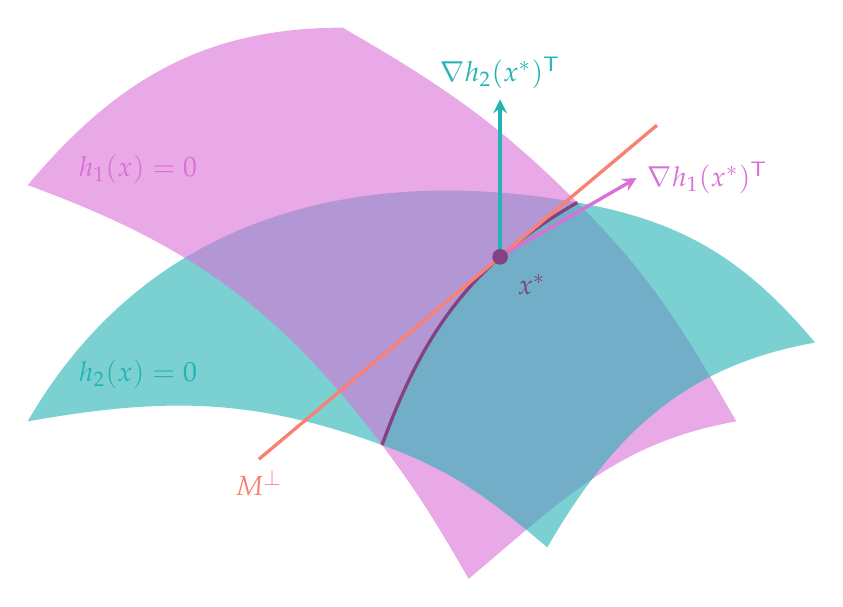
\begin{tikzpicture}[very thick,>=stealth,scale=2]

    \draw[fill=TealBlue, fill opacity=0.6, draw=none]
    (0, 0) to[out=10, in=160] (2.25,-0.15) to[out=70, in=210] (3.49,1.39) to[out=170, in=60] cycle;
    
    \draw[fill=Orchid, fill opacity=0.6, draw=none]
    (2.25,-0.15) to[out=-53, in=120] (2.8, -1) to [out=40, in=190] (4.5, 0) to[out=120, in=-45] (3.49,1.39) to[out=210, in=70] cycle;

    \draw[fill=TealBlue, fill opacity=0.6, draw=none] (2.25,-0.15) to[out=-20, in=140] (3.3, -0.8) to [out=60, in=190] (5, 0.5) to[out=130, in=-10] (3.49,1.39) to[out=210, in=70] cycle;

    \draw[fill=Orchid, fill opacity=0.6, draw=none]
    (0,1.5) to[out=-20, in=127] (2.25, -0.15) to [out=70, in=210] (3.49, 1.39) to[out=135, in=-30] (2,2.5) to [out=180, in=50] cycle;

    \newcommand{\intersectcolor}{black!40!Orchid}

    \draw[\intersectcolor] (2.25, -0.15) to[out=70, in=210] (3.49, 1.39);

    \node[Orchid] at (0.7, 1.6) {$h_1(x)=0$};
    \node[TealBlue] at (0.7, 0.3) {$h_2(x)=0$};
    
    \draw[Salmon] (3,1.045) -- ++(40:1.3);
    \draw[Salmon] (3,1.045) -- ++(220:2) node[below] {$M^\perp$};

    \draw[Orchid,->] (3,1.045) -- ++(30:1) node[right] {$\nabla h_1(x^*)^\t$};
    \draw[TealBlue,->] (3,1.045) -- ++(90:1) node[above] {$\nabla h_2(x^*)^\t$};

    \node[fill=\intersectcolor,draw=none,label={below right:\textcolor{\intersectcolor}{$x^*$}},circle,inner sep=2pt] at (3,1.045) {};
\end{tikzpicture}
\end{document}
